\documentclass[11pt,a4paper]{article}

% ----------------------------- Paquetes -----------------------------
\usepackage[utf8]{inputenc}
\usepackage[spanish]{babel}
\usepackage[T1]{fontenc}
\usepackage[margin=2.7cm]{geometry}
\usepackage{amsmath,amssymb,mathtools}
\usepackage{graphicx}
\usepackage{booktabs}
\usepackage{algorithm}
\usepackage{algpseudocode}
\usepackage{fancyhdr}
\usepackage{xcolor}
\usepackage[colorlinks=true,linkcolor=blue!50!black,citecolor=blue!50!black,urlcolor=blue!50!black]{hyperref}
\usepackage{caption}
\usepackage{enumitem}

\renewcommand{\arraystretch}{1.15}

\pagestyle{fancy}
\fancyhf{}
\fancyhead[L]{Aproximaci\'on RBF multicu\'adrica con selecci\'on greedy}
\fancyhead[R]{\thepage}
\renewcommand{\headrulewidth}{0.4pt}

\newcommand{\R}{\mathbb{R}}
\newcommand{\Phimat}{\boldsymbol{\Phi}}
\newcommand{\wvec}{\mathbf{w}}
\newcommand{\yvec}{\mathbf{y}}

\title{\Large \textbf{Aproximaci\'on de datos experimentales dispersos mediante \\
redes de funciones de base radial (RBF) multicu\'adricas: \\
marco te\'orico, algoritmo y validaci\'on}}

\author{Reporte t\'ecnico}
\date{\today}

\begin{document}

\maketitle

\begin{abstract}
\noindent
Se presenta el dise\~no de un modelo de aproximaci\'on basado en funciones de
base radial (RBF, \emph{Radial Basis Functions}) con n\'ucleo multicu\'adrico,
orientado a un problema de regresi\'on con $N=84$ observaciones experimentales,
$d=5$ variables independientes y una variable dependiente, en presencia de
ruido de medici\'on no despreciable. Dado el car\'acter disperso de los datos
(pocos puntos en un espacio de dimensi\'on relativamente alta) y su naturaleza
ruidosa, el modelo combina cuatro ingredientes: (i) estandarizaci\'on de las
variables independientes, (ii) regularizaci\'on de Tikhonov (\emph{ridge})
sobre los pesos radiales, (iii) selecci\'on \emph{greedy} de centros guiada
por un estimador anal\'itico del error de validaci\'on cruzada
\emph{leave-one-out} (LOOCV), calculado mediante la f\'ormula de Rippa/Allen
sin necesidad de reajustar el modelo $N$ veces, y (iv) b\'usqueda en grilla
de los hiperpar\'ametros (par\'ametro de forma $c$ y coeficiente de
regularizaci\'on $\lambda$). Se documenta el marco te\'orico completo,
la derivaci\'on de la f\'ormula de LOOCV eficiente, el algoritmo propuesto
y su validaci\'on num\'erica sobre datos sint\'eticos con estructura y
nivel de ruido comparable al problema real.
\end{abstract}

\tableofcontents

% =====================================================================
\section{Introducci\'on y planteamiento del problema}
% =====================================================================

Se dispone de un conjunto de $N = 84$ observaciones experimentales de la forma
\[
\left(x_1^{(i)}, x_2^{(i)}, x_3^{(i)}, x_4^{(i)}, x_5^{(i)}, z^{(i)}\right),
\qquad i = 1, \dots, N,
\]
que se interpreta como muestras ruidosas de una funci\'on subyacente desconocida
\[
z = f(x_1, x_2, x_3, x_4, x_5) + \varepsilon,
\]
donde $\varepsilon$ representa el error experimental (ruido de medici\'on). El
objetivo es construir un modelo $\hat f: \R^5 \to \R$ que aproxime $f$ a partir
de estas observaciones, siendo utilizable tanto para interpolaci\'on dentro del
dominio muestreado como, con las debidas reservas, para predicci\'on en puntos
cercanos no observados.

El problema presenta dos dificultades que condicionan cada decisi\'on de
dise\~no del modelo:

\begin{enumerate}[label=(\alph*)]
    \item \textbf{Dispersi\'on de los datos (\emph{sparsity}).} Con $N=84$
    puntos en un espacio de $d=5$ dimensiones, la densidad efectiva de
    muestreo por dimensi\'on es baja. Este es el efecto conocido como
    \emph{maldici\'on de la dimensionalidad} (\emph{curse of dimensionality}):
    el volumen del espacio de entrada crece exponencialmente con $d$, mientras
    que el n\'umero de datos permanece fijo, de modo que las regiones del
    dominio quedan, en promedio, pobremente muestreadas.

    \item \textbf{Ruido experimental.} Al tratarse de datos de ensayo, cada
    observaci\'on $z^{(i)}$ contiene un componente de error no despreciable.
    Esto descarta, de entrada, cualquier esquema de \textbf{interpolaci\'on
    exacta} (que fuerza $\hat f(x^{(i)}) = z^{(i)}$ para todo $i$): un
    interpolante exacto reproducir\'ia el ruido junto con la se\~nal,
    produciendo un modelo con m\'inima varianza aparente en entrenamiento pero
    p\'esima capacidad de generalizaci\'on.
\end{enumerate}

Estas dos condiciones motivan el uso de una red RBF regularizada, con
selecci\'on de centros guiada expl\'icitamente por una estimaci\'on de error
de generalizaci\'on (no de error de entrenamiento), como se detalla en las
secciones siguientes.

% =====================================================================
\section{Marco te\'orico}
% =====================================================================

\subsection{Funciones de base radial (RBF)}

Una funci\'on de base radial es una funci\'on $\phi: \R_{\ge 0} \to \R$ que
depende \'unicamente de la distancia (norma eucl\'idea) entre un punto de
evaluaci\'on $\mathbf{x} \in \R^d$ y un \emph{centro} $\mathbf{c}_j \in \R^d$:
\[
\phi_j(\mathbf{x}) = \phi\!\left(\lVert \mathbf{x} - \mathbf{c}_j \rVert\right)
= \phi(r), \qquad r = \lVert \mathbf{x} - \mathbf{c}_j \rVert .
\]

Un modelo RBF aproxima la funci\'on objetivo como una combinaci\'on lineal de
estas funciones centradas en un conjunto de puntos $\{\mathbf{c}_1, \dots,
\mathbf{c}_M\}$:
\[
\hat f(\mathbf{x}) = \sum_{j=1}^{M} w_j\, \phi\!\left(\lVert \mathbf{x} -
\mathbf{c}_j \rVert\right) + p(\mathbf{x}),
\]
donde $p(\mathbf{x})$ es, opcionalmente, un polinomio de bajo grado (t\'ipicamente
constante o lineal) cuyo rol se explica en la secci\'on~\ref{subsec:cpd}.

La elecci\'on del n\'ucleo $\phi$ determina las propiedades de aproximaci\'on
del modelo. En este trabajo se emplea el n\'ucleo \textbf{multicu\'adrico}:
\[
\boxed{\; \phi(r) = \sqrt{r^2 + c^2} \;}
\]
donde $c > 0$ es el \emph{par\'ametro de forma} (\emph{shape parameter}).
A diferencia de n\'ucleos como el gaussiano $\phi(r) = e^{-r^2/c^2}$, la
multicu\'adrica es una funci\'on \textbf{no acotada y mon\'otona creciente} en
$r$: no decae a cero lejos del centro, lo que le confiere mejor comportamiento
num\'erico (matrices menos mal condicionadas en muchos reg\'imenes) y una
capacidad de aproximaci\'on global reconocida emp\'iricamente como muy buena
incluso con relativamente pocos centros \cite{buhmann2003,hardy1971,franke1982}.

\subsection{Funciones condicionalmente definidas positivas y el t\'ermino
polinomial}
\label{subsec:cpd}

La multicu\'adrica \textbf{no} es una funci\'on definida positiva en el sentido
cl\'asico (Bochner), sino \textbf{condicionalmente definida positiva de orden
1} \cite{micchelli1986}. Esto significa que la matriz $\Phimat$ con entradas
$\Phimat_{ij} = \phi(\lVert \mathbf{c}_i - \mathbf{c}_j\rVert)$ no es, en
general, definida positiva sobre todo $\R^M$, sino \'unicamente sobre el
subespacio de vectores $\mathbf{v}$ que satisfacen la restricci\'on lineal
$\sum_i v_i = 0$.

La consecuencia pr\'actica cl\'asica (en el problema de interpolaci\'on exacta,
sin regularizaci\'on) es que, para garantizar que el sistema lineal sea
resoluble de forma \'unica, es necesario a\~nadir un t\'ermino polinomial
$p(\mathbf{x})$ de grado acorde al orden de condicionalidad (una constante,
para orden 1) y una restricci\'on de ortogonalidad de la forma
$\sum_j w_j\, q(\mathbf{c}_j) = 0$ para todo polinomio $q$ de ese grado
\cite{micchelli1986,buhmann2003}.

En el presente trabajo, dado que el ajuste es \textbf{regularizado} (no es
interpolaci\'on exacta), se opta por una relajaci\'on pr\'actica y ampliamente
usada en la literatura de redes RBF \cite{chen1991}: se incorpora una cola
polinomial de grado~1 (constante m\'as t\'erminos lineales)
\[
p(\mathbf{x}) = \beta_0 + \sum_{k=1}^{d} \beta_k x_k,
\]
\textbf{sin} penalizaci\'on de regularizaci\'on sobre los coeficientes
$\beta_k$, y \textbf{sin} imponer la restricci\'on de ortogonalidad estricta.
Este t\'ermino cumple dos funciones: (i) captura la tendencia global lineal
de los datos, aliviando a la parte radial de tener que modelarla, y (ii)
mejora sustancialmente el comportamiento del modelo fuera de la envolvente
convexa de los datos de entrenamiento (extrapolaci\'on), donde las RBF puras
tienden a producir valores poco confiables.

\subsection{Estandarizaci\'on de las variables independientes}

Como $\phi$ depende de la distancia eucl\'idea $\lVert \mathbf{x}-\mathbf{c}_j
\rVert$, la escala relativa de las variables $x_1,\dots,x_5$ afecta
directamente la forma del modelo: si una variable tiene un rango num\'erico
mucho mayor que las dem\'as, la distancia queda dominada por esa variable y
las dem\'as se vuelven, en la pr\'actica, irrelevantes para el n\'ucleo. Por
ello, antes de cualquier c\'alculo de distancias se estandariza cada variable
(transformaci\'on \emph{z-score}):
\[
\tilde x_k = \frac{x_k - \mu_k}{\sigma_k}, \qquad
\mu_k = \frac{1}{N}\sum_{i=1}^N x_k^{(i)}, \qquad
\sigma_k = \sqrt{\frac{1}{N}\sum_{i=1}^N \left(x_k^{(i)}-\mu_k\right)^2},
\]
para $k=1,\dots,5$. Todas las distancias, centros y evaluaciones del modelo se
realizan en este espacio estandarizado; las predicciones sobre nuevos puntos
se obtienen aplicando la misma transformaci\'on (con los $\mu_k,\sigma_k$
estimados en el conjunto de entrenamiento).

\subsection{Regularizaci\'on de Tikhonov (regresi\'on \emph{ridge})}
\label{subsec:ridge}

Dado un conjunto fijo de $M$ centros, la matriz de dise\~no
$\Phimat \in \R^{N\times(M+d+1)}$ se construye evaluando el n\'ucleo (y la
cola polinomial) en cada punto de entrenamiento:
\[
\Phimat_{i,\,\cdot} = \Big[\, 1,\; \tilde x_1^{(i)}, \dots, \tilde
x_5^{(i)},\; \phi\big(\lVert \tilde{\mathbf{x}}^{(i)}-\mathbf{c}_1\rVert\big),
\dots, \phi\big(\lVert \tilde{\mathbf{x}}^{(i)}-\mathbf{c}_M\rVert\big)\Big].
\]

El ajuste por m\'inimos cuadrados ordinarios, $\wvec = \arg\min_\wvec
\lVert \Phimat \wvec - \yvec\rVert^2$, interpola exactamente cuando $M=N$ y
es propenso al sobreajuste incluso para $M<N$ si los centros est\'an muy
pr\'oximos entre s\'i (columnas de $\Phimat$ casi colineales). Para
estabilizar el ajuste y penalizar soluciones con pesos radiales grandes
(t\'ipicamente asociadas a oscilaciones esp\'ureas ajustadas al ruido), se
emplea regularizaci\'on de Tikhonov \cite{hoerl1970,tikhonov1977}:
\[
\wvec = \arg\min_{\wvec} \; \lVert \Phimat \wvec - \yvec \rVert^2
\; + \; \lambda \sum_{j \,\in\, \text{radiales}} w_j^2 ,
\qquad \lambda \ge 0,
\]
donde la suma de penalizaci\'on corre \textbf{solo} sobre los pesos asociados
a las funciones radiales, dejando sin penalizar los coeficientes $\beta_k$ de
la cola polinomial (consistente con la pr\'actica est\'andar de no penalizar
t\'erminos de tendencia determin\'istica). Definiendo la matriz diagonal de
penalizaci\'on
\[
P = \operatorname{diag}(\underbrace{0,\dots,0}_{d+1},\underbrace{\lambda,\dots,\lambda}_{M}),
\]
la soluci\'on en forma cerrada es
\[
\wvec = \big(\Phimat^{\!\top}\Phimat + P\big)^{-1} \Phimat^{\!\top}\yvec
\;\equiv\; A^{-1}\Phimat^{\!\top}\yvec, \qquad A := \Phimat^{\!\top}\Phimat + P.
\]

El par\'ametro $\lambda$ controla el equilibrio sesgo--varianza: $\lambda\to0$
recupera m\'inimos cuadrados sin restricciones (bajo sesgo, alta varianza);
$\lambda\to\infty$ fuerza $\wvec\to\mathbf{0}$ (alto sesgo, baja varianza).
El valor \'optimo se determina emp\'iricamente mediante validaci\'on cruzada
(secci\'on~\ref{subsec:loocv}).

\subsection{Sobreajuste y el \emph{trade-off} sesgo--varianza}
\label{subsec:biasvar}

El \textbf{error de entrenamiento},
$\text{RMSE}_{\text{train}} = \sqrt{\tfrac1N\sum_i (z^{(i)}-\hat
f(\mathbf{x}^{(i)}))^2}$, mide qu\'e tan bien el modelo reproduce los mismos
datos usados para ajustarlo. Este error es una funci\'on \textbf{mon\'otona no
creciente} de la complejidad del modelo (n\'umero de centros $M$, o
$1/\lambda$): agregar m\'as centros, o reducir $\lambda$, nunca puede empeorar
el ajuste a los datos observados, y en el l\'imite de interpolaci\'on exacta
($M=N$, $\lambda=0$) el error de entrenamiento es id\'enticamente cero.

Sin embargo, un error de entrenamiento nulo no implica un buen modelo: si el
modelo tiene suficiente flexibilidad para pasar exactamente por cada punto
observado, tambi\'en pasar\'a exactamente por el \emph{ruido} de cada punto,
produciendo oscilaciones esp\'ureas entre observaciones que no reflejan la
funci\'on subyacente $f$. Este fen\'omeno, el \textbf{sobreajuste}
(\emph{overfitting}), es especialmente severo en el problema aqu\'i tratado
por la combinaci\'on de pocos datos, alta dimensionalidad y ruido no
despreciable.

La cantidad relevante para elegir la complejidad del modelo es el
\textbf{error de generalizaci\'on}: el error esperado sobre datos \emph{no
vistos} durante el ajuste. Como no se dispone de un conjunto de prueba
independiente adicional (dado que $N=84$ es ya reducido), este error se
estima mediante validaci\'on cruzada.

\subsection{Validaci\'on cruzada \emph{leave-one-out} (LOOCV)}
\label{subsec:loocv}

La validaci\'on cruzada \emph{leave-one-out} consiste en, para cada
observaci\'on $i=1,\dots,N$: (1) ajustar el modelo usando las $N-1$
observaciones restantes; (2) predecir en el punto $i$ excluido,
$\hat f_{(-i)}(\mathbf{x}^{(i)})$; (3) registrar el residuo
$e_i^{\text{LOO}} = z^{(i)} - \hat f_{(-i)}(\mathbf{x}^{(i)})$. El error de
validaci\'on cruzada se resume como
\[
\text{RMSE}_{\text{LOOCV}} = \sqrt{\frac{1}{N}\sum_{i=1}^{N} \big(
e_i^{\text{LOO}}\big)^2 } .
\]

Como cada predicci\'on $\hat f_{(-i)}(\mathbf{x}^{(i)})$ se genera con un
modelo que \textbf{nunca vio} la observaci\'on $i$, $\text{RMSE}_{\text{LOOCV}}$
es un estimador (aproximadamente) insesgado del error de generalizaci\'on, y
--a diferencia del error de entrenamiento-- \textbf{no} es mon\'otono en la
complejidad del modelo: t\'ipicamente decrece al agregar los primeros centros
(el modelo captura estructura real de $f$) y luego crece de nuevo cuando el
modelo comienza a memorizar el ruido de la muestra espec\'ifica. El m\'inimo
de esta curva en forma de ``U'' identifica la complejidad de modelo que mejor
equilibra sesgo y varianza dados los datos disponibles.

Implementado de forma directa (\emph{fuerza bruta}), LOOCV exige $N$ ajustes
completos del modelo por cada configuraci\'on de hiperpar\'ametros
$(c,\lambda,M)$ evaluada. Dado que el algoritmo aqu\'i propuesto eval\'ua un
n\'umero muy grande de configuraciones (b\'usqueda en grilla de $c$ y
$\lambda$, combinada con selecci\'on greedy de hasta $M$ centros, probando en
cada paso todos los candidatos restantes), el c\'osto de fuerza bruta resulta
prohibitivo. La secci\'on siguiente presenta el resultado cl\'asico que
permite calcular $\text{RMSE}_{\text{LOOCV}}$ de forma \textbf{exacta} con un
\'unico ajuste sobre todos los datos.

\subsection{C\'alculo anal\'itico de LOOCV: f\'ormula de Rippa / Allen (PRESS)}
\label{subsec:rippa}

\subsubsection{Resultado y notaci\'on}

Sea $\hat{\yvec} = \Phimat\wvec = H\yvec$ el vector de valores ajustados con
\textbf{todos} los $N$ datos, donde
\[
H = \Phimat A^{-1} \Phimat^{\!\top}, \qquad A = \Phimat^{\!\top}\Phimat + P,
\]
es la \textbf{matriz de influencia} (\emph{hat matrix}). Sea $e_i = z^{(i)} -
\hat z^{(i)}$ el residuo ordinario (con el modelo completo) y $h_{ii} =
H_{ii}$ la $i$-\'esima entrada diagonal de $H$ (el \emph{leverage} o
``autoinfluencia'' del punto $i$: cu\'anto influye $z^{(i)}$ sobre su propia
predicci\'on $\hat z^{(i)}$). Entonces el residuo \emph{leave-one-out} exacto
satisface
\[
\boxed{\; e_i^{\text{LOO}} = \dfrac{e_i}{1-h_{ii}} \;}
\qquad i = 1,\dots,N.
\]

Este resultado fue establecido por Allen \cite{allen1974} en el contexto
general de regresi\'on lineal (como el estad\'istico PRESS), y fue popularizado
espec\'ificamente para la selecci\'on del par\'ametro de forma en
interpolaci\'on RBF por Rippa \cite{rippa1999}, qui\'en lo formul\'o para el
caso particular de interpolaci\'on \textbf{exacta} (sin regularizaci\'on,
$M=N$) en la forma equivalente
\[
e_i^{\text{LOO}} = \frac{w_i}{\left(\Phimat^{-1}\right)_{ii}},
\]
usando directamente los pesos de interpolaci\'on $w_i$ y la diagonal de la
matriz inversa $\Phimat^{-1}$. Esta forma alternativa es necesaria en el caso
de interpolaci\'on exacta porque all\'i $e_i \equiv 0$ y $h_{ii} \equiv 1$
para todo $i$ (el modelo reproduce cada dato exactamente), de modo que la
expresi\'on general $e_i/(1-h_{ii})$ resulta en una indeterminaci\'on $0/0$.
En el presente trabajo, al emplearse regularizaci\'on ($\lambda>0$), se evita
este caso degenerado y se utiliza directamente la forma general de
Allen/Rippa, $e_i^{\text{LOO}}=e_i/(1-h_{ii})$.

\subsubsection{Derivaci\'on}

Se presenta la derivaci\'on completa por ser el resultado central que hace
computacionalmente viable el algoritmo propuesto.

Sea $\phi_i^{\!\top}$ la $i$-\'esima fila de $\Phimat$ (de modo que
$\Phimat^{\!\top}\Phimat = \sum_{j=1}^N \phi_j\phi_j^{\!\top}$). Al excluir la
observaci\'on $i$, la nueva matriz normal es una actualizaci\'on de
\textbf{rango 1}:
\[
A_{(-i)} = A - \phi_i \phi_i^{\!\top}.
\]
Por la f\'ormula de Sherman--Morrison \cite{golub2013},
\[
A_{(-i)}^{-1} = A^{-1} + \frac{A^{-1}\phi_i\phi_i^{\!\top} A^{-1}}
{1 - \phi_i^{\!\top} A^{-1}\phi_i}
= A^{-1} + \frac{\mathbf{g}\,\mathbf{g}^{\!\top}}{1-h_{ii}}, \qquad
\mathbf{g} := A^{-1}\phi_i,
\]
donde se us\'o que $h_{ii} = \phi_i^{\!\top} A^{-1}\phi_i$. El vector de
pesos ajustado sin la observaci\'on $i$ es
\[
\wvec_{(-i)} = A_{(-i)}^{-1}\Big(\Phimat^{\!\top}\yvec - \phi_i z^{(i)}\Big).
\]
Expandiendo, usando $A^{-1}\Phimat^{\!\top}\yvec = \wvec$ (el ajuste completo),
$\mathbf{g}^{\!\top}\Phimat^{\!\top}\yvec = \phi_i^{\!\top}\wvec = \hat
z^{(i)}$, y $\mathbf{g}^{\!\top}\phi_i = h_{ii}$, tras simplificar t\'erminos
se obtiene
\[
\wvec_{(-i)} = \wvec - \mathbf{g}\,\frac{z^{(i)}-\hat z^{(i)}}{1-h_{ii}}
= \wvec - \mathbf{g}\,\frac{e_i}{1-h_{ii}} .
\]
La predicci\'on en el punto exclu\'ido, usando este nuevo vector de pesos, es
\[
\hat z^{(i)}_{(-i)} = \phi_i^{\!\top}\wvec_{(-i)}
= \hat z^{(i)} - h_{ii}\,\frac{e_i}{1-h_{ii}} .
\]
Finalmente, el residuo \emph{leave-one-out} resulta
\[
e_i^{\text{LOO}} = z^{(i)} - \hat z^{(i)}_{(-i)}
= e_i + h_{ii}\frac{e_i}{1-h_{ii}}
= e_i\left(\frac{1-h_{ii}+h_{ii}}{1-h_{ii}}\right)
= \frac{e_i}{1-h_{ii}},
\]
que es el resultado enunciado. $\blacksquare$

\subsubsection{C\'alculo num\'ericamente estable de $h_{ii}$}
\label{subsec:cholesky}

La expresi\'on $h_{ii} = \phi_i^{\!\top} A^{-1}\phi_i$ podr\'ia calcularse
formando expl\'icitamente $A^{-1}$ y luego la matriz completa $H = \Phimat
A^{-1}\Phimat^{\!\top}$, extrayendo despu\'es su diagonal. Sin embargo, este
enfoque es innecesariamente costoso: forma una matriz $N\times N$ completa
cuando solo se requieren sus $N$ entradas diagonales, y la inversi\'on
expl\'icita de matrices amplifica el n\'umero de condici\'on, siendo menos
estable num\'ericamente que resolver sistemas triangulares
\cite{golub2013,trefethen1997}.

En su lugar, se factoriza $A$ por Cholesky ($A = LL^{\!\top}$, v\'alida por
ser $A$ sim\'etrica y definida positiva para $\lambda>0$), y se observa que
\[
h_{ii} = \phi_i^{\!\top} A^{-1}\phi_i = \phi_i^{\!\top} L^{-\top}L^{-1}\phi_i
= \big\lVert L^{-1}\phi_i \big\rVert^2 .
\]
Definiendo $V^{\!\top} := L^{-1}\Phimat^{\!\top}$ (obtenido resolviendo un
\'unico sistema triangular $LV^{\!\top}=\Phimat^{\!\top}$ con los $N$ lados
derechos simult\'aneamente), se obtiene toda la diagonal de $H$ como
\[
h_{ii} = \sum_{k} V_{ki}^2,
\]
es decir, la suma de cuadrados de la columna $i$ de $V^{\!\top}$. El vector de
pesos $\wvec = A^{-1}\Phimat^{\!\top}\yvec$ se obtiene, sin invertir $A$, con
dos sustituciones triangulares adicionales ($L\mathbf{z}=\Phimat^{\!\top}
\yvec$, luego $L^{\!\top}\wvec = \mathbf{z}$). Este procedimiento evita tanto
la inversi\'on expl\'icita de $A$ como la formaci\'on de $H$ completa.

Se verific\'o emp\'iricamente (Secci\'on~\ref{subsec:validacion_numerica}) que
este c\'alculo coincide con LOOCV por fuerza bruta hasta precisi\'on num\'erica
de m\'aquina, y que la ganancia en tiempo de c\'omputo frente al enfoque por
inversi\'on expl\'icita es despreciable a la escala del problema tratado
($N=84$) pero se vuelve sustancial (varias veces m\'as r\'apido) para
conjuntos de datos de miles de puntos.

\subsection{Selecci\'on \emph{greedy} de centros}
\label{subsec:greedy}

\subsubsection{Motivaci\'on}

En principio, cada uno de los $N=84$ puntos de entrenamiento es un candidato
v\'alido para ser centro de una funci\'on radial. Usar los $N$ puntos como
centros del modelo (interpolaci\'on/regresi\'on completa) es una opci\'on,
pero no necesariamente la mejor: adem\'as del riesgo de sobreajuste ya
discutido, un n\'umero menor de centros produce un modelo m\'as simple,
interpretable y de menor costo de evaluaci\'on, sin sacrificar precisi\'on si
los centros se eligen adecuadamente.

El problema de seleccionar el subconjunto \'optimo de $M$ centros de entre $N$
candidatos es combinatorio ($\binom{N}{M}$ posibilidades) y por tanto
intratable por b\'usqueda exhaustiva. La soluci\'on adoptada es una
\textbf{heur\'istica greedy} (voraz): construir el subconjunto de centros de
forma incremental, agregando en cada paso el candidato que produce la mayor
mejora en un criterio dado, sin reconsiderar decisiones previas.

\subsubsection{Antecedente: m\'inimos cuadrados ortogonales (OLS)}

El algoritmo greedy cl\'asico para selecci\'on de centros en redes RBF es el
m\'etodo de \textbf{m\'inimos cuadrados ortogonales} (\emph{Orthogonal Least
Squares}, OLS) de Chen, Cowan y Grant \cite{chen1991}. En su formulaci\'on
original, en cada iteraci\'on se ortogonaliza (v\'ia Gram-Schmidt) la columna
de cada candidato restante contra las columnas ya seleccionadas, y se elige
el candidato cuya componente ortogonal explica la mayor proporci\'on de la
varianza a\'un no explicada del vector objetivo (el llamado \emph{error
reduction ratio}, ERR). Este esquema es elegante porque la ortogonalizaci\'on
incremental evita reajustar el sistema completo en cada paso.

\subsubsection{Criterio adoptado en este trabajo}

El criterio ERR cl\'asico persigue minimizar el error de \textbf{entrenamiento}
en cada paso, lo cual --como se discuti\'o en la
Secci\'on~\ref{subsec:biasvar}-- no es el objetivo correcto cuando los datos
son ruidosos: perseguir la m\'axima reducci\'on de error de entrenamiento en
cada paso conducir\'ia, sin un criterio de parada adecuado, a agregar todos
los centros disponibles.

En este trabajo se adapta el esquema greedy reemplazando el criterio de
selecci\'on: en cada iteraci\'on, para cada candidato $x_k$ a\'un no
seleccionado, se eval\'ua el $\text{RMSE}_{\text{LOOCV}}$ (Secciones
\ref{subsec:loocv}--\ref{subsec:rippa}) del modelo resultante de agregar $x_k$
al conjunto de centros actual, y se selecciona el candidato que produce el
\textbf{menor} $\text{RMSE}_{\text{LOOCV}}$. El proceso se detiene (criterio
de parada temprana) cuando ning\'un candidato restante mejora el
$\text{RMSE}_{\text{LOOCV}}$ actual en al menos una tolerancia
$\delta_{\min}$, evitando as\'i que el algoritmo agregue centros que solo
mejorar\'ian el ajuste a los datos observados sin mejorar --de hecho,
empeorando-- la capacidad de generalizaci\'on estimada.

El pseudoc\'odigo completo se presenta en el Algoritmo~\ref{alg:greedy}.

\begin{algorithm}[H]
\caption{Selecci\'on greedy de centros guiada por LOOCV}
\label{alg:greedy}
\begin{algorithmic}[1]
\Require Datos estandarizados $\{(\tilde{\mathbf x}^{(i)}, z^{(i)})\}_{i=1}^N$;
par\'ametro de forma $c$; regularizaci\'on $\lambda$; m\'aximo de centros
$M_{\max}$; tolerancia $\delta_{\min}$
\Ensure Conjunto de centros seleccionados $\mathcal{S}$
\State $\mathcal{S} \gets \emptyset$; \quad $\mathcal{R} \gets \{1,\dots,N\}$
\quad (candidatos restantes)
\State $\text{LOOCV}_{\text{mejor}} \gets +\infty$
\While{$\mathcal{R} \neq \emptyset$ \textbf{y} $|\mathcal{S}| < M_{\max}$}
    \For{\textbf{cada} candidato $k \in \mathcal{R}$}
        \State Construir $\Phimat$ con centros $\mathcal{S}\cup\{k\}$
        \State Calcular $\text{RMSE}_{\text{LOOCV}}(k)$ v\'ia f\'ormula de
        Rippa/Allen (Alg.~\ref{alg:rippa})
    \EndFor
    \State $k^\ast \gets \arg\min_{k\in\mathcal{R}} \text{RMSE}_{\text{LOOCV}}(k)$
    \If{$|\mathcal{S}|>0$ \textbf{y} $\text{LOOCV}_{\text{mejor}} -
    \text{RMSE}_{\text{LOOCV}}(k^\ast) < \delta_{\min}$}
        \State \textbf{romper} (detenci\'on temprana: no hay mejora significativa)
    \EndIf
    \State $\mathcal{S} \gets \mathcal{S} \cup \{k^\ast\}$; \quad
    $\mathcal{R} \gets \mathcal{R}\setminus\{k^\ast\}$
    \State $\text{LOOCV}_{\text{mejor}} \gets \text{RMSE}_{\text{LOOCV}}(k^\ast)$
\EndWhile
\State \Return $\mathcal{S}$
\end{algorithmic}
\end{algorithm}

\begin{algorithm}[H]
\caption{C\'alculo de $\text{RMSE}_{\text{LOOCV}}$ (f\'ormula de Rippa/Allen)}
\label{alg:rippa}
\begin{algorithmic}[1]
\Require Matriz de dise\~no $\Phimat$; objetivo $\yvec$; regularizaci\'on
$\lambda$; \'indice $n_{u}$ de columnas no penalizadas
\Ensure $\wvec$, $\text{RMSE}_{\text{train}}$, $\text{RMSE}_{\text{LOOCV}}$
\State $P \gets \operatorname{diag}(0,\dots,0,\lambda,\dots,\lambda)$
\Comment{ceros en las primeras $n_u$ entradas}
\State $A \gets \Phimat^{\!\top}\Phimat + P$
\State $L \gets \text{Cholesky}(A)$ \Comment{$A = LL^{\!\top}$}
\State Resolver $L\mathbf z = \Phimat^{\!\top}\yvec$, luego $L^{\!\top}\wvec =
\mathbf z$ \Comment{sin invertir $A$}
\State Resolver $LV^{\!\top} = \Phimat^{\!\top}$ \Comment{$N$ lados derechos
simult\'aneos}
\State $h_{ii} \gets \sum_k V_{ki}^2$ para $i=1,\dots,N$
\State $\mathbf{e} \gets \yvec - \Phimat\wvec$
\State $\mathbf{e}^{\text{LOO}} \gets \mathbf{e} \,/\, (1-\mathbf h)$
\Comment{divisi\'on elemento a elemento}
\State \Return $\wvec$, $\lVert\mathbf e\rVert/\sqrt N$,
$\lVert\mathbf e^{\text{LOO}}\rVert/\sqrt N$
\end{algorithmic}
\end{algorithm}

\subsection{B\'usqueda de hiperpar\'ametros}

El modelo depende de dos hiperpar\'ametros continuos: el par\'ametro de forma
$c$ de la multicu\'adrica y el coeficiente de regularizaci\'on $\lambda$.
Ambos se seleccionan mediante \textbf{b\'usqueda en grilla}
(\emph{grid search}) sobre rangos log-espaciados,
\[
c \in \{c_1,\dots,c_{n_c}\} \subset [c_{\min}, c_{\max}], \qquad
\lambda \in \{\lambda_1,\dots,\lambda_{n_\lambda}\} \subset
[\lambda_{\min},\lambda_{\max}],
\]
ejecutando, para cada combinaci\'on $(c,\lambda)$, el procedimiento greedy
completo (Algoritmo~\ref{alg:greedy}) y registrando el
$\text{RMSE}_{\text{LOOCV}}$ final alcanzado. Se retiene la combinaci\'on
$(c^\ast,\lambda^\ast)$ y el conjunto de centros $\mathcal{S}^\ast$ que
produce el menor $\text{RMSE}_{\text{LOOCV}}$ global. Gracias a que cada
evaluaci\'on individual usa la f\'ormula anal\'itica de Rippa/Allen (en vez de
LOOCV por fuerza bruta), esta b\'usqueda --que involucra t\'ipicamente
cientos de miles de evaluaciones de modelo-- resulta computacionalmente
factible en un tiempo del orden de un minuto para $N=84$.

% =====================================================================
\section{Metodolog\'ia propuesta: algoritmo completo}
% =====================================================================

Integrando los elementos de la secci\'on anterior, el procedimiento completo
de ajuste es el siguiente:

\begin{enumerate}
    \item \textbf{Preprocesamiento.} Estandarizar las cinco variables
    independientes (z-score) usando media y desviaci\'on est\'andar
    calculadas sobre el conjunto de entrenamiento.

    \item \textbf{B\'usqueda en grilla.} Para cada combinaci\'on
    $(c,\lambda)$ en la grilla:
    \begin{enumerate}
        \item Ejecutar la selecci\'on greedy de centros
        (Algoritmo~\ref{alg:greedy}), guiada por $\text{RMSE}_{\text{LOOCV}}$
        calculado v\'ia la f\'ormula de Rippa/Allen (Algoritmo~\ref{alg:rippa}).
        \item Registrar el $\text{RMSE}_{\text{LOOCV}}$ final y el conjunto de
        centros resultante.
    \end{enumerate}

    \item \textbf{Selecci\'on del modelo final.} Elegir $(c^\ast,\lambda^\ast,
    \mathcal S^\ast)$ como la combinaci\'on de menor $\text{RMSE}_{\text{LOOCV}}$
    entre todas las evaluadas.

    \item \textbf{Ajuste final.} Con los centros $\mathcal S^\ast$ (en el
    espacio estandarizado) y los hiperpar\'ametros \'optimos, resolver
    \[
    \wvec^\ast = \big(\Phimat^{\!\top}\Phimat + P^\ast\big)^{-1}
    \Phimat^{\!\top}\yvec
    \]
    (v\'ia Cholesky, Secci\'on~\ref{subsec:cholesky}) sobre \textbf{todos} los
    $N=84$ datos.

    \item \textbf{Predicci\'on.} Para un punto nuevo $\mathbf x_{\text{new}}$:
    estandarizar con los $\mu_k,\sigma_k$ del entrenamiento, construir la fila
    de dise\~no correspondiente y evaluar $\hat z = \Phimat_{\text{new}}
    \wvec^\ast$.
\end{enumerate}

Este procedimiento queda encapsulado, en la implementaci\'on de referencia, en
la clase \texttt{RBFApproximator} (m\'etodos \texttt{fit} y \texttt{predict}),
sobre el m\'odulo \texttt{rbf\_multiquadric.py}.

% =====================================================================
\section{Resultados experimentales}
% =====================================================================

Con el fin de validar el comportamiento del algoritmo sin depender a\'un de
los datos experimentales reales del ensayo, se gener\'o un conjunto sint\'etico
con la misma estructura del problema real: $N=84$ observaciones, $d=5$
variables independientes muestreadas uniformemente en $[-2,2]^5$, una funci\'on
subyacente no lineal con interacciones entre variables,
\[
f(\mathbf x) = \sin(x_1) + 0.5\,x_2^2 - x_3 x_4 + 0.3\,x_5 +
0.2\cos(x_1 x_5),
\]
y ruido aditivo Gaussiano de desviaci\'on est\'andar igual al $15\%$ de la
desviaci\'on est\'andar de $f$ sobre la muestra, $\varepsilon \sim
\mathcal N(0,\, (0.15\,\sigma_f)^2)$.

\subsection{Convergencia de la selecci\'on greedy y calidad del ajuste}

La Figura~\ref{fig:diagnosticos} resume el comportamiento del modelo ajustado
mediante el procedimiento completo (b\'usqueda en grilla + greedy + ajuste
final). El panel superior izquierdo muestra la curva de convergencia del
$\text{RMSE}_{\text{LOOCV}}$ durante la selecci\'on greedy: decrece con las
primeras incorporaciones de centros y se estabiliza (activando el criterio de
parada temprana) alrededor de $M=28$ centros de los $84$ candidatos
disponibles. Los paneles restantes muestran, respectivamente, el ajuste
predicho contra el valor real ($R^2 \approx 0.988$ sobre el conjunto de
entrenamiento completo), los residuos en funci\'on del valor predicho (sin
patrones sistem\'aticos evidentes) y la distribuci\'on de dichos residuos.

\begin{figure}[htbp]
    \centering
    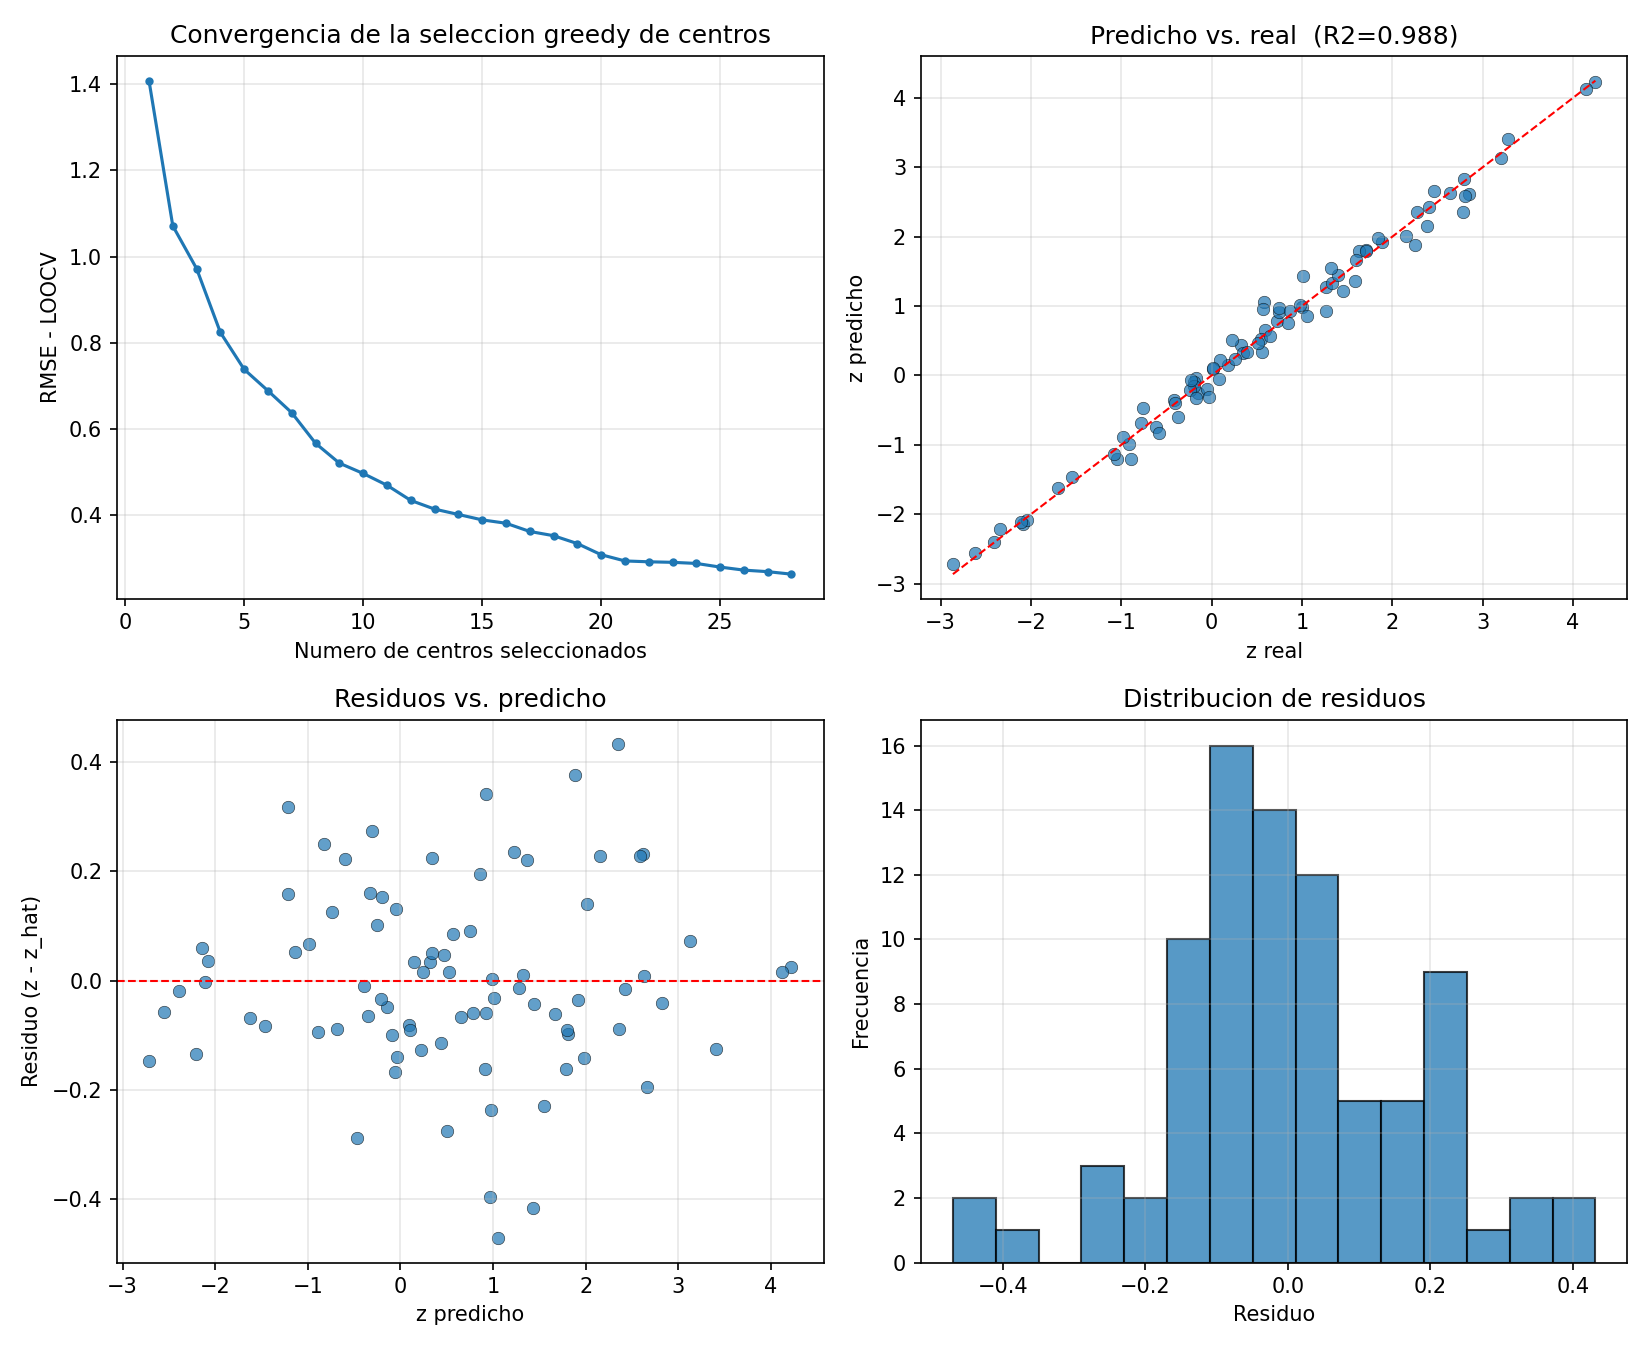
\includegraphics[width=0.92\textwidth]{figs/diagnosticos_rbf.png}
    \caption{Diagn\'osticos del modelo ajustado sobre el conjunto sint\'etico
    de validaci\'on: convergencia del LOOCV durante la selecci\'on greedy
    (arriba-izq.), valores predichos vs.\ observados (arriba-der.), residuos
    vs.\ predicho (abajo-izq.) y distribuci\'on de residuos (abajo-der.).}
    \label{fig:diagnosticos}
\end{figure}

\subsection{Curvas de dependencia parcial}

Para explorar el efecto marginal de cada variable independiente, la
Figura~\ref{fig:dependencia} presenta, para cada $x_k$, la predicci\'on del
modelo al variar $x_k$ en su rango observado mientras las dem\'as variables se
fijan en su valor medio. Estas curvas son un corte unidimensional de una
superficie de respuesta de cinco dimensiones y, por construcci\'on, no
capturan efectos de \textbf{interacci\'on} entre variables (por ejemplo, el
t\'ermino $-x_3 x_4$ de la funci\'on generadora no se manifiesta claramente en
los paneles individuales de $x_3$ y $x_4$, precisamente porque su efecto
depende conjuntamente de ambas variables).

\begin{figure}[htbp]
    \centering
    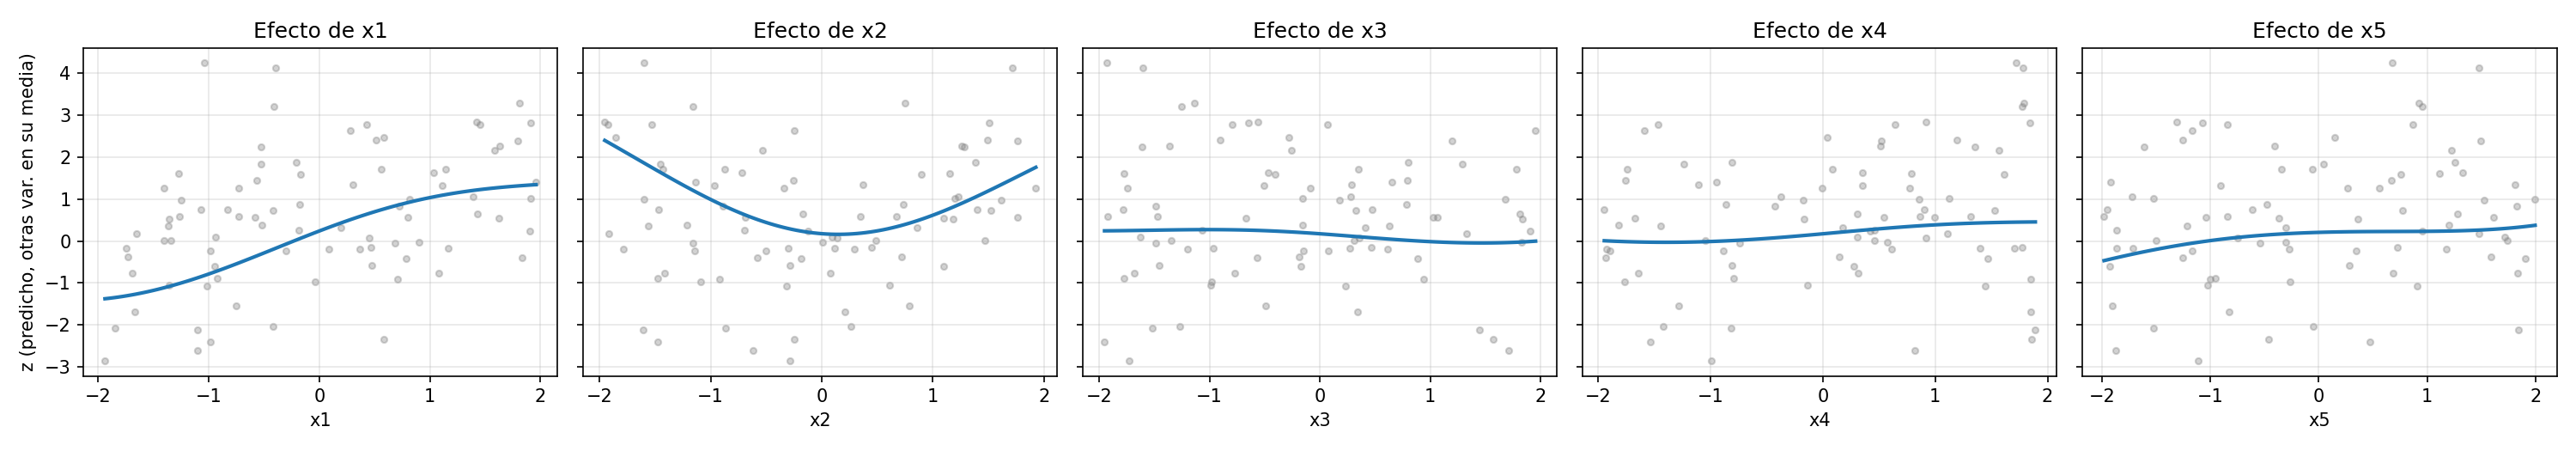
\includegraphics[width=\textwidth]{figs/dependencia_parcial_rbf.png}
    \caption{Curvas de dependencia parcial del modelo ajustado para cada una
    de las cinco variables independientes (con las dem\'as fijas en su media
    muestral). Los puntos grises son los datos observados, proyectados sobre
    cada eje.}
    \label{fig:dependencia}
\end{figure}

\subsection{Error de entrenamiento vs.\ error LOOCV: evidencia emp\'irica del
sobreajuste}

Para ilustrar expl\'icitamente el argumento te\'orico de la
Secci\'on~\ref{subsec:biasvar}, se repiti\'o la selecci\'on greedy
\textbf{sin} criterio de parada temprana (forzando la incorporaci\'on de los
$84$ centros disponibles) y con una regularizaci\'on deliberadamente casi nula
($\lambda=10^{-8}$), registrando en cada paso tanto
$\text{RMSE}_{\text{train}}$ como $\text{RMSE}_{\text{LOOCV}}$. La
Figura~\ref{fig:trainvsloocv} muestra el resultado en dos escalas: un
acercamiento a los primeros $45$ centros (panel izquierdo) y el rango
completo en escala logar\'itmica (panel derecho).

\begin{figure}[htbp]
    \centering
    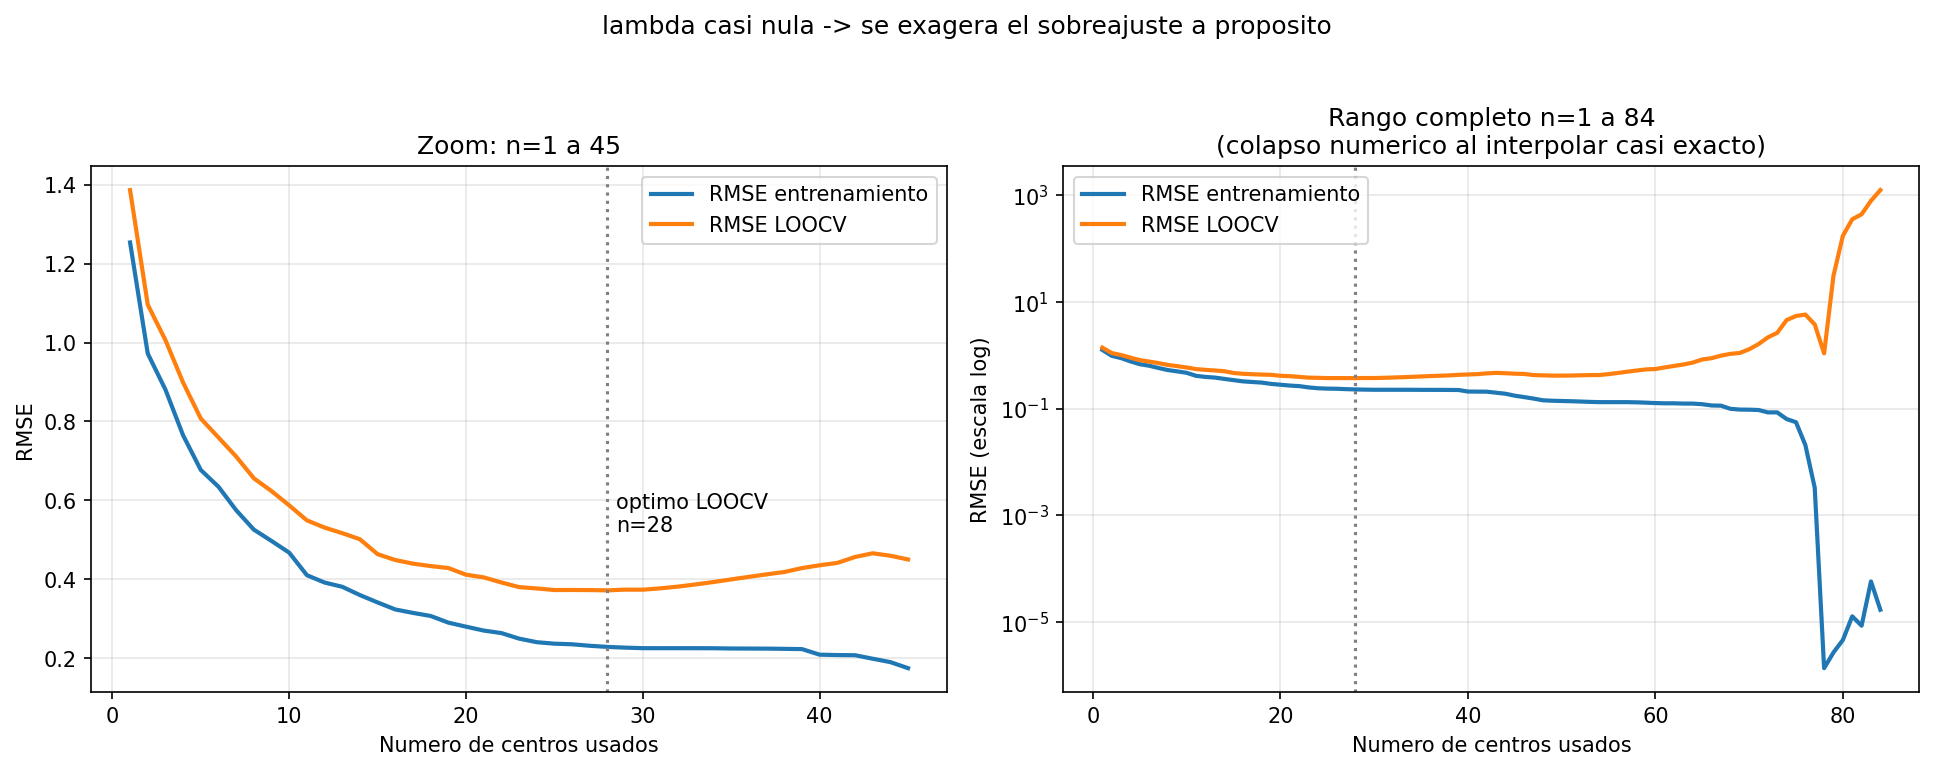
\includegraphics[width=\textwidth]{figs/train_vs_loocv.png}
    \caption{Evoluci\'on del error de entrenamiento y del error LOOCV en
    funci\'on del n\'umero de centros incorporados, con regularizaci\'on casi
    nula ($\lambda=10^{-8}$) para exagerar deliberadamente el efecto de
    sobreajuste. El error de entrenamiento decrece mon\'otonamente hasta
    valores num\'ericamente nulos ($\sim 10^{-5}$) al aproximarse a la
    interpolaci\'on exacta ($M=N=84$), mientras que el error LOOCV, tras un
    m\'inimo cercano a $M=28$, crece de nuevo y eventualmente diverge por
    la casi-singularidad num\'erica asociada a $h_{ii}\to 1$.}
    \label{fig:trainvsloocv}
\end{figure}

El comportamiento observado es exactamente el previsto por la teor\'ia: el
error de entrenamiento es mon\'otono decreciente en la complejidad del modelo,
mientras que el error LOOCV exhibe la forma de ``U'' caracter\'istica del
compromiso sesgo--varianza, con m\'inimo pr\'acticamente coincidente con el
punto de parada temprana identificado por el Algoritmo~\ref{alg:greedy} en
la Secci\'on anterior ($M\approx 28$--$32$, seg\'un el nivel de regularizaci\'on
usado).

\subsection{Validaci\'on num\'erica de la f\'ormula de Rippa/Allen}
\label{subsec:validacion_numerica}

Se verific\'o la correcci\'on de la implementaci\'on de la
Secci\'on~\ref{subsec:rippa} comparando, sobre un subconjunto de $N=15$ puntos
y $M=15$ centros fijos, el residuo LOOCV calculado (i) anal\'iticamente v\'ia
$e_i/(1-h_{ii})$ y (ii) por fuerza bruta (excluyendo expl\'icitamente cada
observaci\'on, reajustando el modelo con las $N-1$ restantes --manteniendo
fijo el conjunto de centros-- y evaluando en el punto exclu\'ido). Ambos
c\'alculos coincidieron con una diferencia m\'axima absoluta del orden de
$10^{-11}$, consistente con el error num\'erico de punto flotante esperado, lo
que confirma la correcci\'on de la derivaci\'on de la Secci\'on
\ref{subsec:rippa} y de su implementaci\'on.

Un punto sutil que conviene remarcar es que, en esta verificaci\'on por fuerza
bruta, al excluir la observaci\'on $i$ se elimina \'unicamente su
\textbf{ecuaci\'on} (la fila correspondiente en $\Phimat$ y $\yvec$), pero
\textbf{no} su rol como potencial centro (columna de $\Phimat$): los centros
son ubicaciones fijas en el espacio de entrada, independientes de qu\'e
subconjunto de ecuaciones se use para ajustar los pesos. Confundir ambos roles
--como ocurri\'o en un primer intento de verificaci\'on durante el desarrollo
de este trabajo, al eliminar tambi\'en la columna asociada al punto
exclu\'ido-- produce discrepancias del orden de $10^{-2}$--$10^{-1}$ entre el
c\'alculo por fuerza bruta (incorrecto en ese caso) y la f\'ormula anal\'itica,
por estar comparando, de hecho, dos problemas de ajuste distintos.

\subsection{Eficiencia num\'erica: Cholesky vs.\ inversi\'on expl\'icita}

Se compar\'o el tiempo de c\'omputo del Algoritmo~\ref{alg:rippa} implementado
(i) mediante inversi\'on expl\'icita de $A$ y formaci\'on completa de $H$, y
(ii) mediante factorizaci\'on de Cholesky y sustituciones triangulares
(Secci\'on~\ref{subsec:cholesky}), para distintos tama\~nos de problema. Los
resultados se resumen en la Tabla~\ref{tab:cholesky}.

\begin{table}[htbp]
\centering
\caption{Tiempo de c\'omputo por evaluaci\'on de modelo (segundos, promedio
sobre m\'ultiples repeticiones) para ambos m\'etodos, en funci\'on del tama\~no
del problema.}
\label{tab:cholesky}
\begin{tabular}{@{}rrrrr@{}}
\toprule
$N$ (datos) & $n_{cols}$ (centros+cola) & Inversi\'on expl\'icita (s) &
Cholesky (s) & \emph{Speedup} \\
\midrule
84    & 35  & 0.00034 & 0.00032 & 1.07$\times$ \\
300   & 100 & 0.00164 & 0.00109 & 1.51$\times$ \\
1\,000  & 300 & 0.02691 & 0.01379 & 1.95$\times$ \\
3\,000  & 500 & 0.22928 & 0.07738 & 2.96$\times$ \\
8\,000  & 800 & 2.67004 & 0.42996 & 6.21$\times$ \\
\bottomrule
\end{tabular}
\end{table}

A la escala del problema tratado en este trabajo ($N=84$), la diferencia de
tiempo entre ambos enfoques es despreciable (los tiempos est\'an dominados por
el costo fijo de las llamadas a las rutinas de \'algebra lineal, no por el
n\'umero de operaciones de punto flotante). La ventaja del enfoque basado en
Cholesky se vuelve sustancial \'unicamente a partir de conjuntos de datos de
varios cientos o miles de puntos. No obstante, se adopt\'o el enfoque de
Cholesky como pr\'actica por defecto en la implementaci\'on de referencia, por
su mayor estabilidad num\'erica (evita amplificar el n\'umero de condici\'on
asociado a la inversi\'on expl\'icita), independientemente de la ganancia en
velocidad.

% =====================================================================
\section{Limitaciones y recomendaciones}
% =====================================================================

\begin{itemize}
    \item \textbf{Maldici\'on de la dimensionalidad.} Con $N=84$ observaciones
    en $d=5$ dimensiones, la densidad efectiva de muestreo es baja. Los
    resultados de generalizaci\'on (estimados por LOOCV) deben interpretarse
    con cautela, especialmente en regiones del dominio alejadas de los datos
    observados.

    \item \textbf{Extrapolaci\'on.} Aunque la cola polinomial lineal mejora el
    comportamiento fuera de la envolvente convexa de los datos, no existe
    garant\'ia de validez de las predicciones en regiones no muestreadas. Se
    recomienda restringir el uso pr\'actico del modelo al rango observado de
    cada variable, o acompa\~nar cualquier extrapolaci\'on de un an\'alisis de
    sensibilidad.

    \item \textbf{Multicolinealidad entre variables independientes.} Si dos o
    m\'as de las cinco variables predictoras est\'an correlacionadas entre
    s\'i, la dimensionalidad efectiva del problema es menor a $5$, lo cual
    podr\'ia mejorar la calidad del ajuste si se detecta y se tiene en cuenta
    (por ejemplo, mediante an\'alisis de componentes principales previo).

    \item \textbf{Comparaci\'on con modelos alternativos.} Se recomienda
    contrastar los resultados del modelo RBF con al menos un modelo de
    referencia m\'as simple (por ejemplo, regresi\'on polinomial de bajo
    grado) y, si se dispone de tiempo de c\'omputo adicional, con un proceso
    Gaussiano (\emph{Gaussian Process Regression}), que modela expl\'icitamente
    el nivel de ruido mediante un t\'ermino de \emph{nugget} y provee, de forma
    natural, intervalos de incertidumbre en la predicci\'on.
\end{itemize}

% =====================================================================
\section{Conclusiones}
% =====================================================================

Se dise\~n\'o e implement\'o un modelo de aproximaci\'on RBF con n\'ucleo
multicu\'adrico adaptado a las condiciones espec\'ificas del problema
planteado: pocos datos experimentales, alta dimensionalidad relativa y ruido
de medici\'on no despreciable. La combinaci\'on de regularizaci\'on de
Tikhonov, selecci\'on greedy de centros guiada por un estimador anal\'itico de
error de generalizaci\'on (LOOCV, v\'ia la f\'ormula de Rippa/Allen) y
b\'usqueda en grilla de hiperpar\'ametros permite obtener un modelo que
equilibra expl\'icitamente ajuste a los datos y capacidad de generalizaci\'on,
sin requerir un conjunto de validaci\'on independiente adicional --algo
particularmente valioso dado el tama\~no reducido de la muestra disponible.

La validaci\'on sobre datos sint\'eticos con estructura comparable al problema
real confirm\'o: (i) que el criterio de selecci\'on basado en LOOCV detiene
correctamente la incorporaci\'on de centros antes de que el modelo comience a
sobreajustarse al ruido; (ii) que la f\'ormula anal\'itica de LOOCV coincide
exactamente con el c\'alculo por fuerza bruta; y (iii) que la implementaci\'on
num\'ericamente estable (Cholesky) reproduce id\'enticos resultados que el
c\'alculo por inversi\'on expl\'icita, con ventajas de velocidad que se
vuelven relevantes solo a mayor escala de datos.

% =====================================================================
\begin{thebibliography}{99}

\bibitem{rippa1999}
Rippa, S. (1999).
\emph{An algorithm for selecting a good value for the parameter c in radial
basis function interpolation}.
Advances in Computational Mathematics, 11(2--3), 193--210.

\bibitem{chen1991}
Chen, S., Cowan, C.\ F.\ N., \& Grant, P.\ M.\ (1991).
\emph{Orthogonal least squares learning algorithm for radial basis function
networks}.
IEEE Transactions on Neural Networks, 2(2), 302--309.

\bibitem{allen1974}
Allen, D.\ M.\ (1974).
\emph{The relationship between variable selection and data augmentation and
a method for prediction}.
Technometrics, 16(1), 125--127.

\bibitem{hoerl1970}
Hoerl, A.\ E., \& Kennard, R.\ W.\ (1970).
\emph{Ridge regression: Biased estimation for nonorthogonal problems}.
Technometrics, 12(1), 55--67.

\bibitem{tikhonov1977}
Tikhonov, A.\ N., \& Arsenin, V.\ Y.\ (1977).
\emph{Solutions of Ill-Posed Problems}.
Winston \& Sons, Washington D.C.

\bibitem{micchelli1986}
Micchelli, C.\ A.\ (1986).
\emph{Interpolation of scattered data: Distance matrices and conditionally
positive definite functions}.
Constructive Approximation, 2(1), 11--22.

\bibitem{buhmann2003}
Buhmann, M.\ D.\ (2003).
\emph{Radial Basis Functions: Theory and Implementations}.
Cambridge University Press.

\bibitem{hardy1971}
Hardy, R.\ L.\ (1971).
\emph{Multiquadric equations of topography and other irregular surfaces}.
Journal of Geophysical Research, 76(8), 1905--1915.

\bibitem{franke1982}
Franke, R.\ (1982).
\emph{Scattered data interpolation: Tests of some methods}.
Mathematics of Computation, 38(157), 181--200.

\bibitem{golub2013}
Golub, G.\ H., \& Van Loan, C.\ F.\ (2013).
\emph{Matrix Computations} (4th ed.).
Johns Hopkins University Press.

\bibitem{trefethen1997}
Trefethen, L.\ N., \& Bau III, D.\ (1997).
\emph{Numerical Linear Algebra}.
SIAM.

\end{thebibliography}

\end{document}
